Building on chapter \ref{chap:introduction}'s definition of an autonomous trading system that integrates market data and sentiment signals to navigate uncertainty and complexity, chapter 2 reviews prior research and foundational concepts supporting our approach. Section \ref{sec:scope} define the scope and boundaries of our \gls{LLM}-augmented reinforcement learning framework.  Next, section \ref{sec:literature} survey two bodies of academic work: deep \gls{RL} for financial trading and \gls{LLM}–based sentiment analysis.  We analyze the strengths and limitations of each and highlight gaps our thesis addresses. Finally, section \ref{sec:mdp} and \ref{sec:sac} introduce the core technical foundations and laying the groundwork for our integrated system.

\section{Scope of Research}
\label{sec:scope}
Our goal is to develop an autonomous stock trading agent that combines advanced \gls{RL} techniques with sentiment signals.  We frame the trading problem as a \gls{MDP} in which the agent observes features of the market and decides on actions (portfolio allocations) to maximize long-term return. The state include historical prices, technical indicators, and crucially, sentiment features derived from textual data (news).  We focus on model-free deep \gls{RL} methods in a continuous-action setting, specifically using the entropy-regularized \gls{SAC} algorithm, due to its stability and exploration benefits.  The environment is assumed to be partially observable and non-stationary, reflecting real market complexity. Key constraints include limited and noisy training data, unpredictable regime shifts, and the need for generalization rather than overfitting.  We do not attempt to model execution details like order matching, nor do we consider alternatives like supervised learning on static data.  Instead, our scope is on the decision-making core: using an RL agent to act continuously in the market, augmented by qualitative signals.

This research deliberately bridges two domains that have often been studied separately.  Traditional quantitative trading models frequently ignore unstructured information, while natural-language methods rarely drive actual trading decisions.  Our focus is on how \gls{LLM}'s sentiment can be incorporated into an \gls{RL} agent's state or reward to guide trading.  We assume that sentiment affects market prices (even with delay) and that the \gls{RL} agent can learn to exploit this. Limitations of our study include reliance on historical backtests (no live trading), restricted asset universes, and a single-agent perspective (not modeling other traders). By clarifying these boundaries, we set the stage for developing and evaluating \gls{LLM}-augmented RL strategies.

\section{Related Works}
\label{sec:literature}
\subsection{Reinforcement Learning in Financial Trading}
Reinforcement learning has attracted considerable interest for quantitative trading, portfolio management, and execution problems. Surveys note that \gls{RL} methods (especially model-free, policy-based and actor-critic methods) have been applied to tasks like order execution, market-making, hedging, and portfolio optimization \cite{Hambly2023}. These works typically frame finance problems as \gls{MDP}s and leverage deep neural networks to approximate value functions and policies \cite{Kabbani2022, Xia2023, Kabbani2022}. Dang explore value-based \gls{RL} algorithm like \gls{DQN} and its variants Double \gls{DQN} and Dueling \gls{DQN} for trading of US-based stocks \cite{Dang2020}. Xia et al. implemented a trading agent using the \gls{PPO} algorithm and custom reward structure that incorporate risk aversion \cite{Xia2023}. Kodurupaka et al. performed a comprehensive analysis comparing \gls{DQN} and \gls{DDPG} using historical data from S\&P 500 \cite{Kodurupaka2024}. However, each has trade-offs. For example, on-policy methods like \gls{PPO} are robust but sample-inefficient and require fresh data for each update, which is costly in finance \cite{Haarnoja2018}. Off-policy methods like \gls{DDPG} can reuse data but have suffered historically from stability issues \cite{Haarnoja2018}. \gls{SAC} has recently emerged as a state-of-the-art deep \gls{RL} algorithm that mitigates these issues via entropy-regularization.

Empirical studies have shown that \gls{RL}-based trading agents can learn complex, non-linear strategies that often outperform simple benchmarks. For example, Jie et al. constructs a \gls{PPO}-based agent augmented with an \gls{LSTM} to capture temporal trends and cost dynamics \cite{Jie2024}. Other recent work applies deep \gls{RL} to crypto markets, leverage, hedging, and other specialized tasks \cite{Qin2024, LiuKang2024}. These studies highlight the advantage of \gls{RL} in optimizing dynamic strategies with minimal model assumptions. In contrast, classical portfolio models rely on fixed formulas that may oversimplify market behavior \cite{Hambly2023}.

Nevertheless, there are well-known challenges. Financial data is noisy, non-stationary, and often limited, which exacerbates \gls{RL}'s sample-complexity and generalization issues. Practitioners warn of severe overfitting: extraordinarily high reported \gls{SR} ratios in some studies likely indicate look-ahead bias or data-snooping \cite{Nikolaos2025}. For instance, \gls{SR} above \(3\) are statistically rare, yet some \gls{RL}] papers claim \gls{SR}s of \(20\)+, raising skepticism about robustness \cite{Nikolaos2025}. Moreover, formulating the trading problem as an \gls{MDP} itself is difficult, so one must select state variables and rewards carefully, and important factors like news or macro shocks are hard to include without exploding dimensionality. Explainability and risk management are also concerns, because many deep-\gls{RL} policies are black-box, and naive maximization of reward can lead to “over-greedy” actions that incur tail risks. Overall, while \gls{RL} offers a powerful framework for sequential decision-making in trading, its practical limitations motivate hybrid approaches.

\subsection{LLMs and Sentiment Analysis in Financial Forecasting}
Independent of \gls{RL}, a large body of work has explored textual sentiment as a predictor of market movements. Traditional approaches used human-crafted sentiment indices or dictionaries  to score news or reports \cite{Loughran2011}. More recently, neural models have taken over. Transformer-based models such as \gls{BERT} have been fine-tuned on financial text to classify sentiment \cite{Kirtac2024, Fatouros2023}. These bidirectional models are optimized for sentiment classification tasks and often achieve good accuracy on labeled datasets.

However, the advent of powerful generative \gls{LLM}s (GPT, LLaMA, etc.) is reshaping the field. Large models pretrained on broad corpora offer deeper contextual understanding and can be used in flexible ways. For example, Fatouros et al. compare ChatGPT (GPT-3.5) to FinBERT on forex news: ChatGPT achieved \(\sim 35\%\) higher classification accuracy and \(36\%\) stronger correlation with actual returns, using only zero-shot prompting \cite{Fatouros2023}. Similarly, Kirtac and Germano find that an OPT (GPT-3) model achieves \(74.4\%\) sentiment accuracy on US news – far above the \(50.1\%\) accuracy of the Loughran–McDonald dictionary \cite{Kirtac2024}. In portfolio tests, strategies based on OPT sentiment also achieved much higher Sharpe ratios (\(3.05\)) than dictionary-based strategies (\(1.23\)). These studies highlight that modern LLMs can capture nuanced tone in financial text that older methods miss.

\gls{LLM}s can be employed in various ways: zero-shot or few-shot prompting, fine-tuning on labeled financial sentiment data, or domain-specific pre-training. Prompt engineering has become an art: for zero-shot classification, one might simply instruct “Label the sentiment of this news headline: ...”. For more complex analysis, Chen et al. implemented a Domain Knowledge Chain-of-Thought strategy to integrate domain specific knowledge with chain-of-thought reasoning \cite{Chen2025}. In parallel, researchers have built finance-specific \gls{LLM}s or adapters (e.g. BloombergGPT, FinGPT, FinLlama) by fine-tuning on financial corpora. Such models combine both the deep linguistic knowledge of \gls{LLM}s and domain-specific vocabulary \cite{Nie2024}.

The advantages of \gls{LLM}-based sentiment analysis are clear: these models capture context and subtleties that lexicons or shallow models cannot \cite{LiuArulappan2024, Kirtac2024}. \gls{GPT} models excel at real-time interpretation of complex news, while \gls{BERT} models provide structured classification ability \cite{LiuArulappan2024}. Empirical evidence shows \gls{LLM}-derived sentiment signals often correlate strongly with future returns \cite{Fatouros2023, Kirtac2024}. Moreover, \gls{LLM}s can handle very long or unstructured texts via summarization. For instance, Chiu and Hung use a LLaMA-2-based summarizer on 10-K filings (MD\&A sections); their \gls{LLM}-derived sentiment signals produced trading strategies with significantly higher buy-and-hold returns than FinBERT-based or traditional methods \cite{Chiu2024}. This suggests that generative AI can “distill” lengthy documents into actionable sentiment.

Nonetheless, \gls{LLM}-based methods also have drawbacks. \gls{LLM}s are computationally intensive and sometimes unpredictable. Without careful prompting or fine-tuning, they may hallucinate or misinterpret financial jargon. Prompted classification can be sensitive to wording and may require domain knowledge to work well \cite{Chen2025}. Domain-specific models like BloombergGPT are proprietary, and open LLMs may still lag in finance-specific accuracy. There is also debate about interpretability: one recent survey notes that \gls{LLM} improve contextual depth but can still be opaque, unlike simple lexicons \cite{Kirtac2024}. In practice, most \gls{LLM}-sentiment studies remain separate from decision-making algorithms. Few prior works have fully integrated news-based \gls{LLM} sentiment into an \gls{RL} decision agent.

This gap motivates our thesis: \gls{LLM}-augmented \gls{RL}. While \gls{RL} can optimize sequential trading strategies, it generally lacks qualitative inputs \cite{Hambly2023}. Conversely, \gls{LLM}s provide powerful sentiment signals but do not themselves make trading decisions. Recent work by Unnikrishnan explicitly combines these: she shows that \gls{RL} models augmented with \gls{LLM}-derived news sentiment earn higher profit and net worth than vanilla \gls{RL} or buy-and-hold strategies \cite{Unnikrishnan2024}. Our work follows this emerging direction. We will leverage the stability and expressiveness of \gls{SAC} for trading, and use \gls{RL} sentiment as part of the state or reward, aiming to capture both quantitative price dynamics and qualitative market mood.

\section{Markov Decision Process}
\label{sec:mdp}
An \gls{MDP} is formally characterized by a tuple \((S, A, P, R, \gamma)\). The first component, \(S\), represents the State Space, encompassing every possible configuration or situation the environment can be in. A state \(s \in S\), in the ideal \gls{MDP} setting, is assumed to capture all relevant information about the environment necessary for making an informed decision at a given time. The nature of these states can be vastly different, from discrete representations like the positions of pieces on a chess board, to high-dimensional, continuous vectors such as the joint angles and velocities of a robotic arm. A critical assumption underpinning the utility of a state within the pure \gls{MDP} framework is that it provides a sufficient statistic of the history. This means that the past sequence of events leading to the current state does not provide additional predictive power beyond what is already encapsulated in the state itself; the future is conditionally independent of the past, given the present state.

Complementing the state space is the Action Space \(A\), which defines the set of all possible actions \(a \in A\) that the agent can execute. Actions are the means by which the agent influences the environment, and like states, they can be discrete or continuous. The definition of the action space fundamentally constrains the capabilities of the agent and can significantly impact the complexity of the learning problem.

The dynamics of the environment, specifying how states evolve in response to actions, are captured by the Transition Probability Function \(P\). This function, \(P(s' | s, a)\), dictates the probability of the environment transitioning to a new state \(s'\) given that the agent is in state \(s\) and takes action \(a\). This probabilistic nature accounts for inherent stochasticity in the environment's response. Crucially, this transition function inherently relies on the Markov Property: the next state \(s'\) depends only on the current state \(s\) and the current action \(a\). Mathematically, this Markov property is expressed as:
\[P(s_{t+1}| s_t, a_t, s_{t-1}, a_{t-1}, ..., s_0, a_0) = P(s_{t+1} | s_t, a_t)\]

The guiding signal for the agent's learning process is provided by the Reward Function \(R\). This function, often denoted as \(R(s, a, s')\), specifies the scalar immediate reward (or penalty) the agent receives after taking action \(a\) in state \(s\) and transitioning to state \(s'\). The overarching goal of the agent is to learn a sequence of actions that maximizes the cumulative sum of these rewards over time. This cumulative reward, known as the return, is often defined as:
\[G_t = \Sigma_{k=0}^\infty \gamma^k r_{t+k+1}\]
where \(\gamma \in [0,1]\) is the discount factor to modulates the importance of future rewards relative to immediate ones, and \(r_t\) is the immediate reward at time step \(t\).

Within this MDP framework, the agent's decision-making mechanism is formalized as a policy \(\pi\):
\[\pi(a|s) = P(a_t = a | s_t = s)\]
which maps states to actions (or distributions over actions). The ultimate aim is to discover an optimal policy \(\pi^*\) that maximizes the expected cumulative discounted reward \(\mathbb{E}[G_t | s_t = s]\) for all state \(s\).

However, the assumption of perfect and complete state observability, central to the \gls{MDP} formulation, is often a ideal assumption that does not hold in many complex, real-world scenarios. More frequently, an agent does not have access to the true underlying state of the environment. Instead, it receives observations that are correlated with the true state but may be noisy, incomplete, or ambiguous. This realistic scenario is formally modeled by a \gls{POMDP}, with Figure \ref{fig:MDP_POMDP} illustrating the crucial difference \cite{Blumenthal2024}.

\begin{figure}
\centering
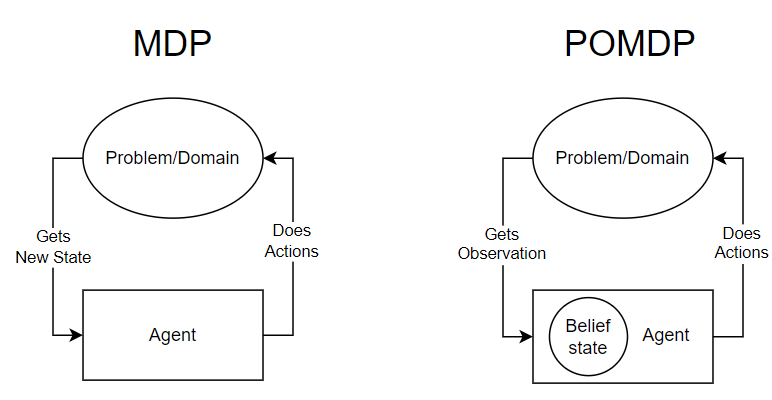
\includegraphics[width=0.8\textwidth]{images/MDP_POMDP_comparison.png}
\caption{Differences between MDP and POMDP. In POMDP, the environment only provide an observation of the true state to the agent.}
\label{fig:MDP_POMDP}
\end{figure}

A \gls{POMDP} extends the \gls{MDP} framework by explicitly acknowledging this imperfect perception. It is typically defined by a tuple \((S, A, P, R, \Omega, O, \gamma)\), where \(S\), \(A\), \(P\), \(R\), and \(\gamma\) are similar to their \gls{MDP} counterparts. The new components are the observation space \(\Omega\), a set of all possible observations \(o \in \Omega\) that the agent can receive from the environment, and the Observation Probability Function \(O(o | s', a)\), which defines the probability of the agent receiving observation \(o\) given that the environment has transitioned to the true state \(s'\) after the agent took action \(a\) in the previous (hidden) state.

In a \gls{POMDP}, since the true state \(s\) is not directly known, the agent cannot base its decisions directly on \(s\). Instead, the agent must operate based on the history of its actions and the observations it has received. To make optimal decisions, an agent in a POMDP often needs to maintain a belief state:
\[b(s_t) = P(s_t | o_t, a_{t-1}, o_{t-1}, ..., a_0, o_0)\]
which is a probability distribution over the set of all possible true states \(S\), representing the belief of the agent about the current true state \(s_t\) given the entire history of past actions and observations up to time \(t\). This belief state can be updated recursively using Bayes' rule:
\[b_t(s') \propto  O(o_t | s', a_{t-1}) \Sigma_{s \in S} P(s' | s, a_{t-1}) b_{t-1}(s)\]
The policy in a \gls{POMDP} thus becomes a mapping from belief states (or, more practically, from histories of observations) to actions: \(\pi(a | b)\) or \(\pi(a | h_t)\) where \(h_t = (o_0, a_0, ..., a_{t-1}, o_t)\) is the observation-action history. Finding an optimal policy in a \gls{POMDP} is significantly more challenging than in an \gls{MDP} because the agent must contend with uncertainty about the true state of the world and potentially infer it from a stream of partial information.

The problem of stock trading, which is the focus of this thesis, serves as an example of a \gls{POMDP}. An \gls{RL} agent attempting to trade stocks does not have access to the complete, true state of the financial market. Factors such as the aggregate sentiment of all market participants, the undisclosed intentions and order books of other traders, unreleased material news, and the true "fair value" of assets remain largely hidden. The agent instead receives observations, such as historical price and volume data, technical indicators, and, in the context of this work, signals derived from \gls{LLM} analyzing news articles, financial reports, and social media.

\section{Soft Actor-Critic}
\label{sec:sac}
In \gls{RL} field, \gls{SAC} stands as a state-of-the-art algorithm, particularly recognized for its efficacy and stability in continuous action spaces, though adaptable to discrete ones as well.What distinguishes \gls{SAC} and contributes significantly to its robust performance is its core principle of maximum entropy reinforcement learning. Instead of solely aiming to maximize the conventional expected cumulative reward, \(\mathbb{E}_\pi[\Sigma_{t=0}^T \gamma^t R(s_t, a_t)]\), \gls{SAC} seeks to find a policy that also maximizes its own entropy at each step.

The inclusion of an entropy term in the objective function profoundly impacts the learning dynamics and the nature of the learned policy. The augmented \gls{SAC} objective function is expressed as:
\[J(\pi) = \mathbb{E}_{s_t \sim \rho_\pi, a_t \sim \pi(\cdot|s_t)} [R(s_t, a_t) + \alpha H(\pi(\cdot|s_t))]\]
Here, \(s_t\) are states visited under policy \(\pi\), \(a_t\) are actions sampled from \(\pi(\cdot|s_t)\), \(R(s_t, a_t)\) is the immediate reward, and the entropy of the policy \(\pi\) in state \(s_t\) is:
\[H(\pi(\cdot|s_t)) = \mathbb{E}_{a_t \sim \pi(\cdot|s_t)}[-log \pi(a_t|s_t)]\]
The temperature parameter \(\alpha > 0\), serves as a crucial trade-off coefficient, determining the relative importance of the entropy bonus compared to the extrinsic reward. A higher \(\alpha\) encourages more stochastic, exploratory behavior by pushing the policy towards a more uniform distribution over actions, while a lower \(\alpha\) shifts the focus more towards exploiting known good actions to maximize rewards. This entropy maximization offers several key advantages: it promotes exploration, which is vital in complex environments with sparse rewards or deceptive local optima; it leads to policies that tend to be more robust to perturbations as they are less committed to a single, deterministic path; and it can accelerate learning by preventing premature convergence to suboptimal strategies.

To implement this maximum entropy objective, \gls{SAC} employs a sophisticated architecture, typically realized using neural networks for function approximation, which comprises several primary, interconnected components. Figure \ref{fig:AC} demonstrates the role of the main component actor and critic in \gls{SAC} agent.

\begin{figure}
\centering
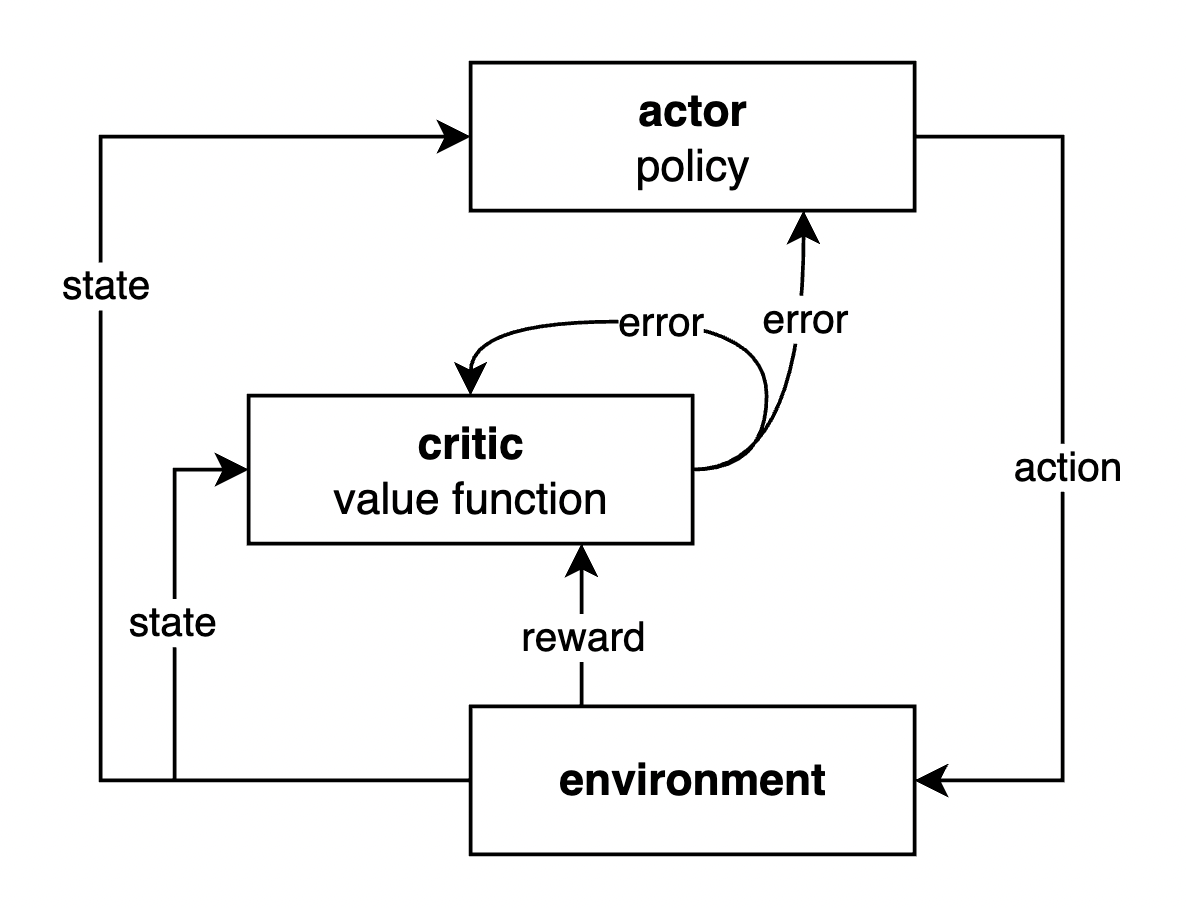
\includegraphics[width=0.8\textwidth]{images/AC_architecture.png}
\caption{Actor-Critic Architecture. The critic is responsible for evaluating the value of the chosen action by estimating the value functions.}
\label{fig:AC}
\end{figure}

First is the Actor, or Policy Network, denoted as \(\pi_\phi(a|s)\) and parameterized by \(\phi\). This network is responsible for learning the agent's behavior. It takes the current state \(s\) as input and outputs the parameters of a probability distribution over the action space. For continuous actions, this is commonly a Gaussian distribution, where the network outputs the mean \(\mu_\phi(s)\) and standard deviation \(\sigma_\phi(s)\). Actions are then stochastically sampled from this distribution during interaction with the environment. The  learning objective of the actor is to choose actions that not only lead to high expected future rewards (as estimated by the critic) but also maintain high policy entropy. To enable gradient-based optimization through the stochastic sampling process, especially in continuous action spaces, \gls{SAC} utilizes the reparameterization trick. This involves expressing the sampled action \(a_t\) as a deterministic function of the policy parameters and an independent noise variable \(\epsilon\):
\[a_t = \mu_\phi(s_t) + \sigma_\phi(s_t) \cdot \epsilon, \quad \epsilon \sim \mathcal{N}(0,I)\]

Second, the Critic component in \gls{SAC} learns one or, more commonly, two Soft Q-Value Networks, \(Q_\theta(s, a)\), parameterized by \(\theta\). These networks learn to estimate the expected sum of future rewards and future entropy bonuses, if the agent starts in state \(s\), takes action \(a\), and subsequently follows the current policy \(\pi\) thereafter. This is known as the soft Q-value. The learning of these Q-functions is guided by a modified Bellman equation that incorporates the entropy term. The target for the soft Q-function is:
\[y(r, s') = r + \gamma(\mathbb{E}_{a' \sim \pi(\cdot|s')} [Q_{target}(s', a')] - \alpha \log \pi(a'|s'))\]
The Q-networks are then trained by minimizing the soft Bellman residual, typically the squared error:
\[L_Q(\theta) = \mathbb{E}_{(s,a,r,s') \sim \mathcal{D}} [(Q_\theta(s,a) - y(r,s'))^2]\]
where \(\mathcal{D}\) is the replay buffer. To combat the overestimation bias common in actor-critic methods, \gls{SAC} often implements the Clipped Double Q-learning technique. This involves learning two independent Q-networks (\(Q_{\theta_1}\) and \(Q_{\theta_2}\)) and using the minimum of their predictions when constructing the target value in the Bellman updates:
\[y(r, s') = r + \gamma(\mathbb{E}_{a' \sim \pi(\cdot|s')} [\min(Q_{target,1}(s', a'), Q_{target,2}(s', a'))] - \alpha \log \pi(a'|s'))\]
This conservative approach helps to mitigate positive bias and generally leads to more stable and reliable value estimates.

Third, to further enhance stability in the learning of the Q-functions, \gls{SAC} utilizes Target Q-Networks (\(Q_{\theta'_1}\) and \(Q_{\theta'_2}\), or \(Q_{target,1}\) and \(Q_{target,2}\) in the equation above) for the critic. These are separate networks whose parameters are periodically or slowly updated copies of the parameter of the main Q-networks. A common update rule is Polyak averaging:
\[\theta'_i \leftarrow \tau\theta_i + (1-\tau)\theta'_i, i=1,2\]
where \(\tau\) is a small constant. By using these slowly changing target networks to calculate the target values in the Bellman equation, the learning process is less prone to oscillations and divergence.

Fourth, a distinctive feature of many \gls{SAC} implementations is the Automated Temperature Parameter \(\alpha\) Tuning. While \(\alpha\) can be set as a fixed hyperparameter, \gls{SAC} often benefits from making \(\alpha\) a learnable parameter. This allows the algorithm to dynamically adjust the emphasis on entropy throughout the learning process, adapting the exploration-exploitation balance. The objective for learning \(\alpha\) is typically to maintain the policy's entropy at a predefined target entropy level \(\mathcal{H}_{target}\) (often set heuristically, e.g., \(-\text{dim}(\mathcal{A})\), where \(\text{dim}(\mathcal{A})\) is the action space dimensionality). This is achieved by performing gradient descent on \(\alpha\) to minimize the objective:
\[L(\alpha) = \mathbb{E}_{a_t \sim \pi(\cdot|s_t)} [-\alpha (\log \pi(a_t|s_t) + \mathcal{H}_{target})]\]

In summary, this chapter formalizes our problem as a \gls{POMDP} in which a \gls{SAC} agent leverages both quantitative market features and \gls{LLM}'s sentiment signals, reviews the strengths and limitations of deep \gls{RL} approaches versus traditional portfolio methods and of modern \gls{LLM}‑based sentiment analysis versus lexicon‑based techniques, and details the theoretical underpinnings of \gls{MDP}s/\gls{POMDP}s and the entropy‑regularized \gls{SAC} algorithm that together provide the foundation for our \gls{LLM}‑augmented trading framework.
